\documentclass[]{article}
\usepackage{lmodern}
\usepackage{amssymb,amsmath}
\usepackage{ifxetex,ifluatex}
\usepackage{fixltx2e} % provides \textsubscript
\ifnum 0\ifxetex 1\fi\ifluatex 1\fi=0 % if pdftex
  \usepackage[T1]{fontenc}
  \usepackage[utf8]{inputenc}
\else % if luatex or xelatex
  \ifxetex
    \usepackage{mathspec}
  \else
    \usepackage{fontspec}
  \fi
  \defaultfontfeatures{Ligatures=TeX,Scale=MatchLowercase}
\fi
% use upquote if available, for straight quotes in verbatim environments
\IfFileExists{upquote.sty}{\usepackage{upquote}}{}
% use microtype if available
\IfFileExists{microtype.sty}{%
\usepackage{microtype}
\UseMicrotypeSet[protrusion]{basicmath} % disable protrusion for tt fonts
}{}
\usepackage[margin=1.5cm]{geometry}
\usepackage{hyperref}
\hypersetup{unicode=true,
            pdftitle={Supplementary Figures},
            pdfauthor={Pierre-Luc Germain},
            pdfborder={0 0 0},
            breaklinks=true}
\urlstyle{same}  % don't use monospace font for urls
\usepackage{natbib}
\bibliographystyle{plainnat}
\usepackage{graphicx,grffile}
\makeatletter
\def\maxwidth{\ifdim\Gin@nat@width>\linewidth\linewidth\else\Gin@nat@width\fi}
\def\maxheight{\ifdim\Gin@nat@height>\textheight\textheight\else\Gin@nat@height\fi}
\makeatother
% Scale images if necessary, so that they will not overflow the page
% margins by default, and it is still possible to overwrite the defaults
% using explicit options in \includegraphics[width, height, ...]{}
\setkeys{Gin}{width=\maxwidth,height=\maxheight,keepaspectratio}
\IfFileExists{parskip.sty}{%
\usepackage{parskip}
}{% else
\setlength{\parindent}{0pt}
\setlength{\parskip}{6pt plus 2pt minus 1pt}
}
\setlength{\emergencystretch}{3em}  % prevent overfull lines
\providecommand{\tightlist}{%
  \setlength{\itemsep}{0pt}\setlength{\parskip}{0pt}}
\setcounter{secnumdepth}{0}
% Redefines (sub)paragraphs to behave more like sections
\ifx\paragraph\undefined\else
\let\oldparagraph\paragraph
\renewcommand{\paragraph}[1]{\oldparagraph{#1}\mbox{}}
\fi
\ifx\subparagraph\undefined\else
\let\oldsubparagraph\subparagraph
\renewcommand{\subparagraph}[1]{\oldsubparagraph{#1}\mbox{}}
\fi

%%% Use protect on footnotes to avoid problems with footnotes in titles
\let\rmarkdownfootnote\footnote%
\def\footnote{\protect\rmarkdownfootnote}

%%% Change title format to be more compact
\usepackage{titling}

% Create subtitle command for use in maketitle
\providecommand{\subtitle}[1]{
  \posttitle{
    \begin{center}\large#1\end{center}
    }
}

\setlength{\droptitle}{-2em}

  \title{Supplementary Figures}
    \pretitle{\vspace{\droptitle}\centering\huge}
  \posttitle{\par}
    \author{Pierre-Luc Germain}
    \preauthor{\centering\large\emph}
  \postauthor{\par}
      \predate{\centering\large\emph}
  \postdate{\par}
    \date{29 Januar, 2020}


\begin{document}
\maketitle

{
\setcounter{tocdepth}{2}
\tableofcontents
}
\newpage

\hypertarget{supplementary-figure-1}{%
\section{Supplementary Figure 1}\label{supplementary-figure-1}}

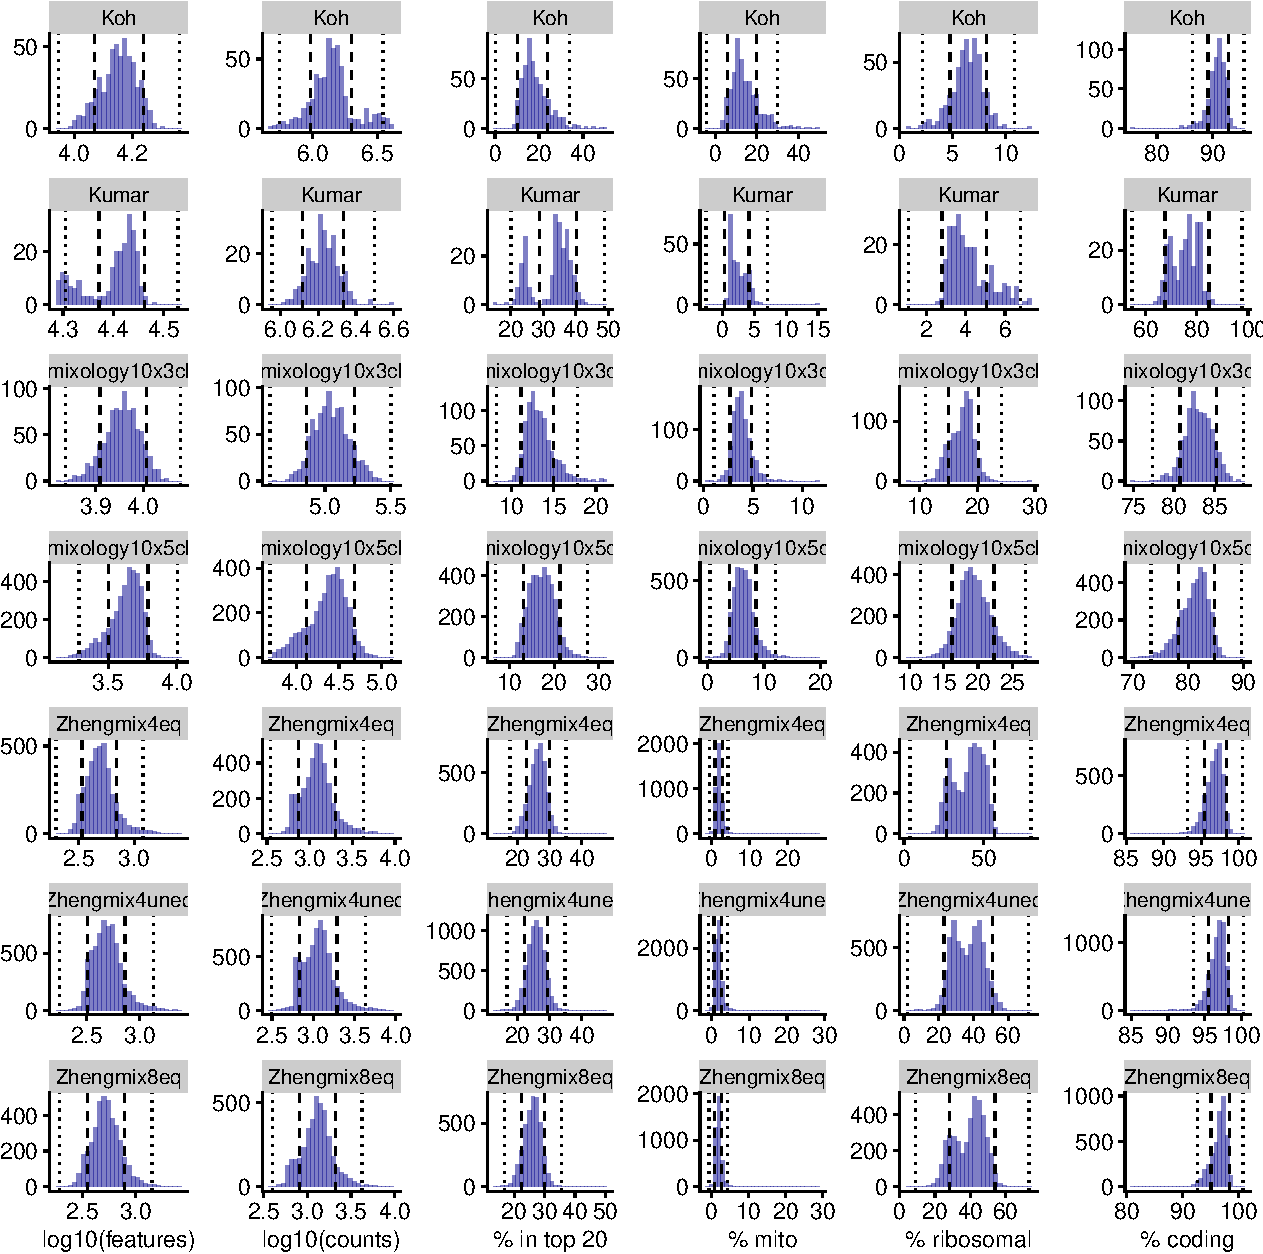
\includegraphics{supp_figures_files/figure-latex/dist_cell_properties-1.pdf}

\hypertarget{supplementary-figure-1-1}{%
\subsubsection{Supplementary Figure 1}\label{supplementary-figure-1-1}}

Distribution across cells of various control properties in the different
datasets. The lines indicate respectively 2 and 5 median absolute
deviations (MADs).

\newpage

\hypertarget{supplementary-figure-2}{%
\section{Supplementary Figure 2}\label{supplementary-figure-2}}

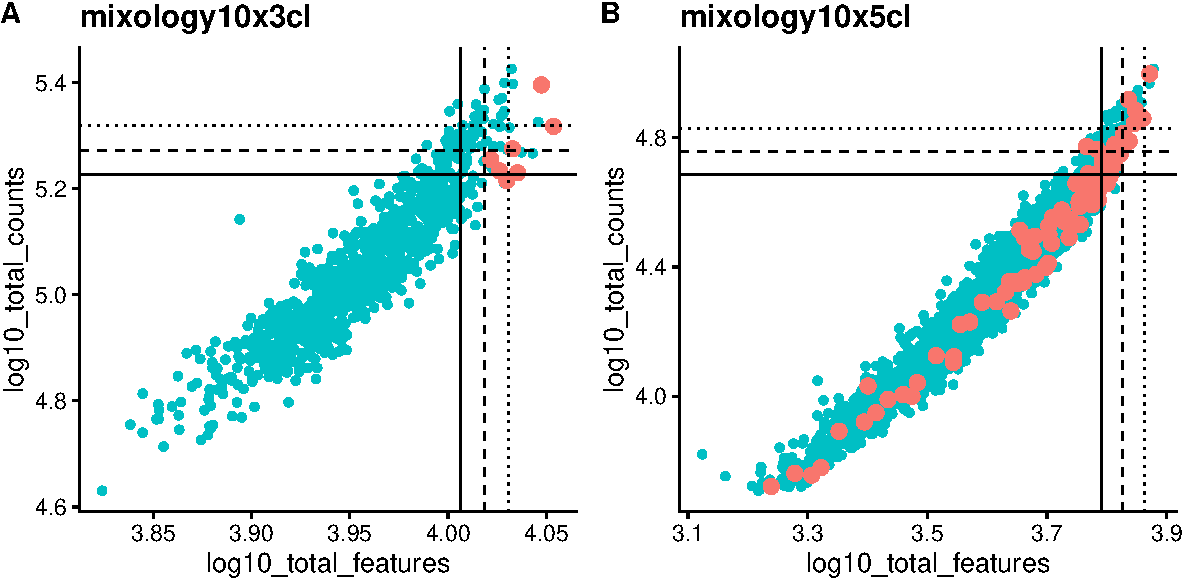
\includegraphics{supp_figures_files/figure-latex/mixology_doublet_featcount-1.pdf}

\hypertarget{supplementary-figure-2-1}{%
\subsubsection{Supplementary Figure 2}\label{supplementary-figure-2-1}}

The total counts and total features per cell of doublets (red) versus
other cells. We used the demuxlet annotation of doublets (based on SNPs)
made available through CellBench. The lines indicate, respectively, 2,
2.5, and 3 median absolute deviations. While doublets tend to have a
higher total count and especially number of detected features, these
features alone are not always sufficient for their identification.

\newpage

\hypertarget{supplementary-figure-3}{%
\section{Supplementary Figure 3}\label{supplementary-figure-3}}

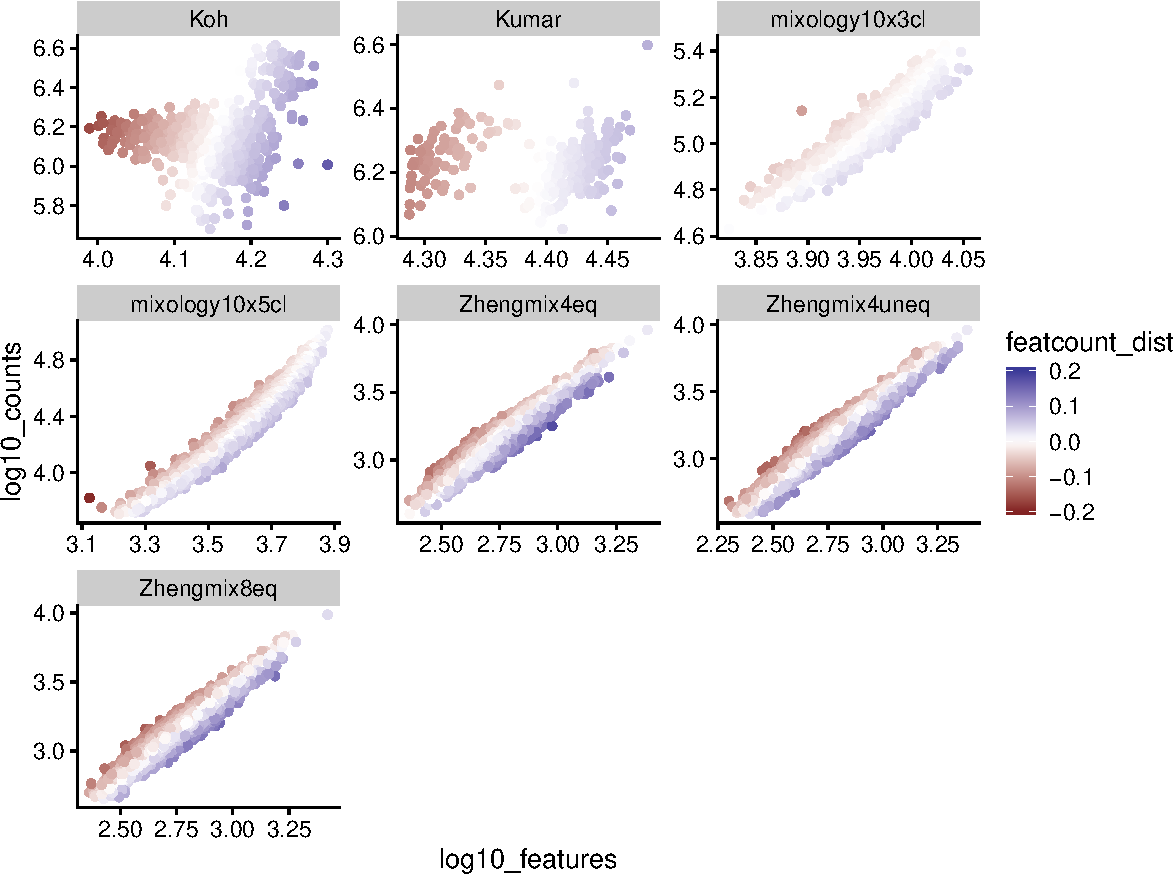
\includegraphics{supp_figures_files/figure-latex/featcount_ratio-1.pdf}

\hypertarget{supplementary-figure-3-1}{%
\subsubsection{Supplementary Figure 3}\label{supplementary-figure-3-1}}

There is a tight relationship, in 10x datasets (i.e.~not the
\texttt{Koh} and \texttt{Kumar} datasets), between the total counts of a
cell and its number of detected features. We therefore include, among
control variables, deviation from this ratio.

\newpage

\hypertarget{supplementary-figure-4}{%
\section{Supplementary Figure 4}\label{supplementary-figure-4}}

\includegraphics{supp_figures_files/figure-latex/cellprops_cor-1.pdf}

\hypertarget{supplementary-figure-4-1}{%
\subsubsection{Supplementary Figure 4}\label{supplementary-figure-4-1}}

There is a tight relationship, in 10x datasets (i.e.~not the
\texttt{Koh} and \texttt{Kumar} datasets), between the total counts of a
cell and its number of detected features. We therefore include, among
control variables, deviation from this ratio.

\newpage

\hypertarget{supplementary-figure-5}{%
\section{Supplementary Figure 5}\label{supplementary-figure-5}}

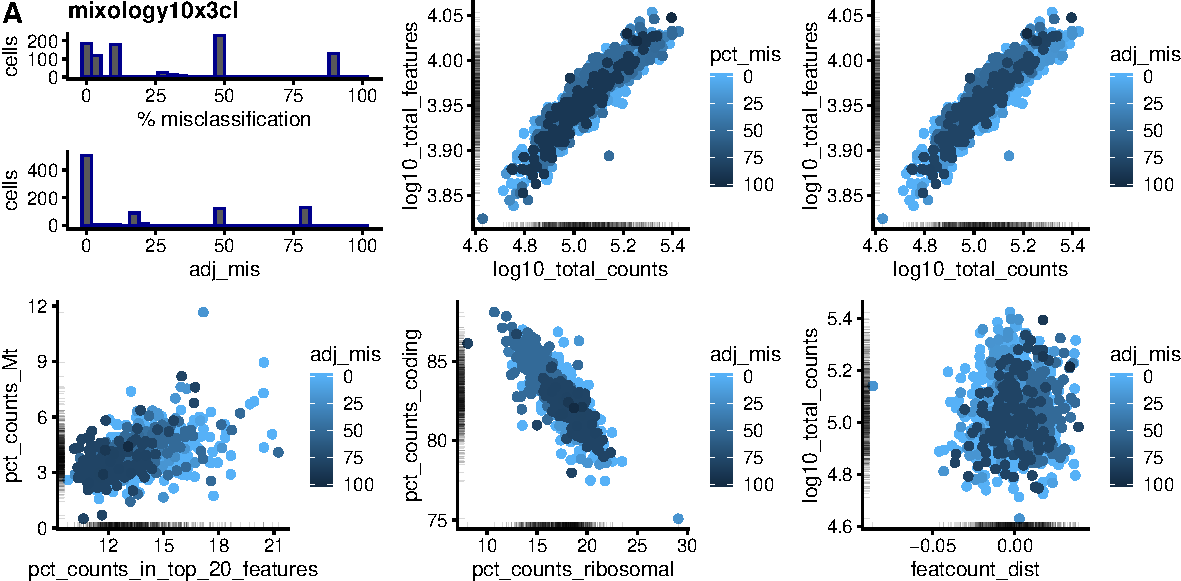
\includegraphics{supp_figures_files/figure-latex/misclass-1.pdf} \vfill
\includegraphics{supp_figures_files/figure-latex/unnamed-chunk-9-1.pdf}

\hypertarget{supplementary-figure-5-1}{%
\subsubsection{Supplementary Figure 5}\label{supplementary-figure-5-1}}

Relationship between various cellular properties and the frequency of
cluster mis-assignment for the mixology10x3cl (A) and mixology10x5cl (B)
datasets. The percentage of misclassification refers to the frequency
with which a given cell is assigned the wrong cluster (using the
Hungarian algorithm for cluster matching) across several hundred
clustering runs with varying parameters. Since some subpopulations tend
to be more misclassified than others, the adjusted rate of
misclassification (\texttt{adj\_mis}) is substracted for the
subpopulation median misclassification rate.

\newpage

\hypertarget{supplementary-figure-6}{%
\section{Supplementary Figure 6}\label{supplementary-figure-6}}

\includegraphics{supp_figures_files/figure-latex/unnamed-chunk-10-1.pdf}
\vfill
\includegraphics{supp_figures_files/figure-latex/unnamed-chunk-11-1.pdf}

\hypertarget{supplementary-figure-6-1}{%
\subsubsection{Supplementary Figure 6}\label{supplementary-figure-6-1}}

Relationship between various cellular properties and the frequency of
cluster mis-assignment for the Zheng equal (A) or unequal (B) mixtures
of four cell types. See Supplementary Figure 5 for more information. The
only clear pattern is that cells with a high number of reads or features
tend to have a higher misclassification rate.

\newpage

\hypertarget{supplementary-figure-7}{%
\section{Supplementary Figure 7}\label{supplementary-figure-7}}

\includegraphics{supp_figures_files/figure-latex/unnamed-chunk-12-1.pdf}

\hypertarget{supplementary-figure-7-1}{%
\subsubsection{Supplementary Figure 7}\label{supplementary-figure-7-1}}

Relationship between various cellular properties and the frequency of
cluster mis-assignment for the Zheng mixture of 8 cell types. See
Supplementary Figure 5 for more information.

\newpage

\hypertarget{supplementary-figure-8}{%
\section{Supplementary Figure 8}\label{supplementary-figure-8}}

\includegraphics{supp_figures_files/figure-latex/filt_more-1.pdf}

\hypertarget{supplementary-figure-8-1}{%
\subsubsection{Supplementary Figure 8}\label{supplementary-figure-8-1}}

Mean clustering F1 score per subpopulation, mean F1 at true number of
clusters, as well as maximum and median proportion of excluded cells per
subpopulation across various filtering strategies. Doublet removal
generally improves clustering accuracy with very mild exclusion rates,
even in datasets that do not have heterotypic doublets. Stringent
distribution-based filtering creates large cell type biases.

\newpage

\hypertarget{supplementary-figure-9}{%
\section{Supplementary Figure 9}\label{supplementary-figure-9}}

\includegraphics{supp_figures_files/figure-latex/unnamed-chunk-15-1.pdf}

\hypertarget{supplementary-figure-9-1}{%
\subsubsection{Supplementary Figure 9}\label{supplementary-figure-9-1}}

Impact of restricting the type of features used on the ARI of the
clustering. \newpage

\hypertarget{supplementary-figure-10}{%
\section{Supplementary Figure 10}\label{supplementary-figure-10}}

\includegraphics{supp_figures_files/figure-latex/norm_nbClusters-1.pdf}

\hypertarget{supplementary-figure-10-1}{%
\subsubsection{Supplementary Figure
10}\label{supplementary-figure-10-1}}

Mean difference between the number of detected clusters and the number
of real subpopulations, depending on the normalization method, the
resolution and the number of dimensions used. The Kumar dataset is not
shown here due to a lack of variation in the number of clusters
detected. A rough ANOVA on
\texttt{nbClusters\textasciitilde{}dataset+norm+dims+resolution}
suggests that seuratvst (sctransform) is associated with a higher number
of clusters (p\textasciitilde{}0.002).

\hypertarget{supplementary-figure-11}{%
\section{Supplementary Figure 11}\label{supplementary-figure-11}}

\includegraphics{supp_figures_files/figure-latex/unnamed-chunk-19-1.pdf}

\hypertarget{supplementary-figure-11-1}{%
\subsubsection{Supplementary Figure
11}\label{supplementary-figure-11-1}}

\textbf{A:} Comparison of the gene-wise proportion of variance explained
by real subpopulations based on Seurat's standard log normalization and
on \texttt{sctransform} variance-stabilizing transformation. Across 10x
datasets, there is a good agreement between the two, the correlation
ranging between 0.92 and 0.97. \textbf{B:} There is also a good
agreement between \emph{variance} and \emph{deviance} explained, with
some genes having a higher deviance explained. \textbf{C-D:}
Relationship between mean expression and the difference between the
proportion of deviance explained and the proportion of variance
explained in two datasets. Genes that have a higher proportion of the
deviance explained than of the variance explained are generally the
lowly-expressed ones.

\newpage

\hypertarget{supplementary-figure-12}{%
\section{Supplementary Figure 12}\label{supplementary-figure-12}}

\begin{verbatim}
## Warning: Removed 328867 rows containing missing values (geom_path).
\end{verbatim}

\begin{verbatim}
## Warning: Removed 302113 rows containing missing values (geom_path).
\end{verbatim}

\begin{verbatim}
## Warning: Removed 101276 rows containing missing values (geom_path).
\end{verbatim}

\begin{verbatim}
## Warning: Removed 68502 rows containing missing values (geom_path).
\end{verbatim}

\begin{verbatim}
## Warning: Removed 94976 rows containing missing values (geom_path).
\end{verbatim}

\begin{verbatim}
## Warning: Removed 101101 rows containing missing values (geom_path).
\end{verbatim}

\begin{verbatim}
## Warning: Removed 96012 rows containing missing values (geom_path).
\end{verbatim}

\includegraphics{supp_figures_files/figure-latex/unnamed-chunk-21-1.pdf}

\hypertarget{supplementary-figure-12-1}{%
\subsubsection{Supplementary Figure
12}\label{supplementary-figure-12-1}}

Proportion of the cumulative \emph{variance} explained by real
subpulations that is retrieved through the selection. For each gene, we
compute the proportion of the variance explained by real subpopulations.
For each rank X, we sum this proportion for the X genes selected by a
given method, and divide it by the sum when selecting the X genes with
the highest variance explained. An ideal selection would therefore be a
horizontal line at 1.

\newpage

\hypertarget{supplementary-figure-13}{%
\section{Supplementary Figure 13}\label{supplementary-figure-13}}

\begin{verbatim}
## Warning: Removed 328867 rows containing missing values (geom_path).
\end{verbatim}

\begin{verbatim}
## Warning: Removed 302113 rows containing missing values (geom_path).
\end{verbatim}

\begin{verbatim}
## Warning: Removed 101276 rows containing missing values (geom_path).
\end{verbatim}

\begin{verbatim}
## Warning: Removed 68502 rows containing missing values (geom_path).
\end{verbatim}

\begin{verbatim}
## Warning: Removed 94976 rows containing missing values (geom_path).
\end{verbatim}

\begin{verbatim}
## Warning: Removed 101101 rows containing missing values (geom_path).
\end{verbatim}

\begin{verbatim}
## Warning: Removed 96012 rows containing missing values (geom_path).
\end{verbatim}

\includegraphics{supp_figures_files/figure-latex/unnamed-chunk-23-1.pdf}

\hypertarget{supplementary-figure-13-1}{%
\subsubsection{Supplementary Figure
13}\label{supplementary-figure-13-1}}

Proportion of the cumulative \emph{deviance} explained by real
subpulations that is retrieved through the selection. For each gene, we
compute the proportion of the variance explained by real subpopulations.
As for Supplementary Figure 12, except using deviance explained.

\newpage

\hypertarget{supplementary-figure-14}{%
\section{Supplementary Figure 14}\label{supplementary-figure-14}}

\includegraphics{supp_figures_files/figure-latex/unnamed-chunk-24-1.pdf}

\hypertarget{supplementary-figure-14-1}{%
\subsubsection{Supplementary Figure
14}\label{supplementary-figure-14-1}}

Clustering accuracy according to the number of genes selected using
various ranking/selection methods. \textbf{A:} Based on sctransform,
\textbf{B:} Based on standard Seurat normalization.

\newpage

\hypertarget{supplementary-figure-15}{%
\section{Supplementary Figure 15}\label{supplementary-figure-15}}

\includegraphics{supp_figures_files/figure-latex/unnamed-chunk-27-1.pdf}

\hypertarget{supplementary-figure-15-1}{%
\subsubsection{Supplementary Figure
15}\label{supplementary-figure-15-1}}

Mean difference between the number of detected clusters and the number
of real subpopulations, depending on the resolution and number of
dimensions used. Based on sctransform and seurat PCA. Increasing the
number of dimensions tends to decrease the number of identified
clusters, especially at resolutions around the default value.

\newpage

\hypertarget{supplementary-figure-16}{%
\section{Supplementary Figure 16}\label{supplementary-figure-16}}

\includegraphics{supp_figures_files/figure-latex/unnamed-chunk-28-1.pdf}

\hypertarget{supplementary-figure-16-1}{%
\subsubsection{Supplementary Figure
16}\label{supplementary-figure-16-1}}

Adjusted Rand Index of clustering depending on the resolution and number
of dimensions used. Based on sctransform and seurat PCA.

\hypertarget{supplementary-figure-17}{%
\section{Supplementary Figure 17}\label{supplementary-figure-17}}

\includegraphics{supp_figures_files/figure-latex/unnamed-chunk-31-1.pdf}

\hypertarget{supplementary-figure-17-1}{%
\subsubsection{Supplementary Figure
17}\label{supplementary-figure-17-1}}

Difference between the number of detected clusters and the number of
real subpopulations according to different clustering paramters.

\newpage

\bibliography{../bmc\_article.bib}


\end{document}
